% ============================================================
%  椰島 (Coconut Island) — 南島椰子主題 beamer theme
%  共用前導檔，供「說明」與「題解」兩份簡報 \input
%  以 XeLaTeX 編譯
% ============================================================
\documentclass[aspectratio=169,12pt]{beamer}

\usepackage{fontspec}
\usepackage{xeCJK}
\usepackage{tikz}
\usepackage{tcolorbox}
\tcbuselibrary{skins}
\usetikzlibrary{shapes.misc,arrows.meta}

% ---- 字型 ----
\setCJKmainfont{Heiti TC}
\setCJKsansfont{Heiti TC}
\setmonofont{JetBrainsMono Nerd Font Mono}
\setsansfont{JetBrainsMono Nerd Font}

% ---- 南島椰子色盤 ----
\definecolor{ocean}{HTML}{0F8B8D}     % 海洋藍綠
\definecolor{deepsea}{HTML}{0A5C5E}   % 深海
\definecolor{sand}{HTML}{F4E4C1}      % 沙灘
\definecolor{coconut}{HTML}{6B4226}   % 椰殼棕
\definecolor{leaf}{HTML}{3A7D44}      % 椰葉綠
\definecolor{sun}{HTML}{F2B705}       % 陽光黃
\definecolor{coral}{HTML}{E07A5F}     % 珊瑚橘
\definecolor{paperbg}{HTML}{FBF6EA}   % 米白底

% ---- Wordle 椰子三色 ----
\definecolor{wgreen}{HTML}{6AAA64}    % 熟椰：對的字母對的位置
\definecolor{wyellow}{HTML}{C9B458}   % 青椰：字母有但位置錯
\definecolor{wgray}{HTML}{787C7E}     % 空殼：沒這個字母

% ---- beamer 外觀 ----
\usetheme{default}
\setbeamertemplate{navigation symbols}{}
\setbeamercolor{background canvas}{bg=paperbg}
\setbeamercolor{frametitle}{bg=ocean,fg=white}
\setbeamercolor{title}{fg=deepsea}
\setbeamercolor{structure}{fg=ocean}
\setbeamercolor{normal text}{fg=coconut!90!black}
\setbeamercolor{itemize item}{fg=leaf}
\setbeamercolor{itemize subitem}{fg=ocean}
\setbeamerfont{frametitle}{series=\bfseries}
\setbeamertemplate{itemize item}{\textcolor{leaf}{\textbf{\textbullet}}}
\setbeamertemplate{itemize subitem}{\textcolor{ocean}{--}}

% 圓角的標題列
\setbeamertemplate{frametitle}{%
  \vspace{0.3em}%
  \begin{beamercolorbox}[wd=\paperwidth,sep=0.45em,leftskip=0.6cm]{frametitle}%
    \textbf{\strut\insertframetitle}%
  \end{beamercolorbox}%
}

% ---- Wordle 方塊 ----
% \tile{顏色}{字母}
\newcommand{\tile}[2]{%
  \tikz[baseline=-0.55ex]{\node[fill=#1,text=white,minimum size=0.92cm,
    inner sep=0pt,font=\bfseries\Large,rounded corners=2pt]{#2};}}
% 一整列五格
\newcommand{\wordrow}[1]{\begin{tikzpicture}[baseline]#1\end{tikzpicture}}

% ---- 小提示框 ----
\newtcolorbox{leafbox}[1][]{%
  enhanced, colback=leaf!8, colframe=leaf, boxrule=1pt, arc=4pt,
  fonttitle=\bfseries, coltitle=white, colbacktitle=leaf, #1}
\newtcolorbox{sunbox}[1][]{%
  enhanced, colback=sun!12, colframe=sun!85!black, boxrule=1pt, arc=4pt,
  fonttitle=\bfseries, coltitle=coconut, colbacktitle=sun, #1}
\newtcolorbox{oceanbox}[1][]{%
  enhanced, colback=ocean!8, colframe=ocean, boxrule=1pt, arc=4pt,
  fonttitle=\bfseries, coltitle=white, colbacktitle=ocean, #1}

% ---- 椰子小圖示 (tikz 畫的椰子) ----
\newcommand{\coconuticon}[1][1]{%
  \begin{tikzpicture}[scale=#1]
    \fill[coconut] (0,0) circle (0.32);
    \fill[coconut!70!black] (-0.1,0.08) circle (0.045);
    \fill[coconut!70!black] (0.1,0.08) circle (0.045);
    \fill[coconut!70!black] (0,-0.05) circle (0.045);
  \end{tikzpicture}}

% ---- 樹根朝天的椰子樹（本年度主題）----
% 畫在原點 (0,0) 為地面，往上長；在 tikzpicture 裡用 scope 平移／縮放：
%   \begin{scope}[shift={(x,y)},scale=s] \upsidedowntree \end{scope}
\newcommand{\upsidedowntree}{%
  % 樹幹：從地面往上
  \draw[line width=3pt, coconut] (0,0)
    .. controls (0.2,0.6) and (-0.05,1.1) .. (0.08,1.55);
  % 樹根朝天：頂端往天空分岔
  \foreach \a/\len in {118/0.5,98/0.62,80/0.6,62/0.48,140/0.4,58/0.34}{
    \draw[line width=1.6pt, coconut!85!black]
      (0.08,1.55) -- ++({\len*cos(\a)},{\len*sin(\a)});}
  % 細根的小分岔
  \foreach \a/\len in {100/0.18,82/0.18,120/0.14,60/0.14}{
    \draw[line width=1pt, coconut!85!black]
      ({0.08+0.5*cos(\a)},{1.55+0.5*sin(\a)}) -- ++({\len*cos(\a+25)},{\len*sin(\a+25)});}
  % 椰葉朝下：從樹冠（下方）往外垂
  \foreach \a in {205,232,258,282,308,335}{
    \draw[line width=2pt, leaf] (0.08,0.55)
      .. controls ({0.08+0.5*cos(\a)},{0.55+0.45*sin(\a)})
         and ({0.08+1.0*cos(\a)},{0.25+0.3*sin(\a)})
      .. ({0.08+1.3*cos(\a)},{0.08});}
  % 椰子：掛在樹冠附近（下方）
  \fill[coconut] (-0.12,0.5) circle (0.12);
  \fill[coconut] (0.3,0.52) circle (0.12);
}



\title{椰島字謎遊戲}
\subtitle{說明簡報}

\begin{document}

% 頁尾：小小的椰子島
\setbeamertemplate{footline}{%
  \hbox{}\hfill
  \raisebox{2pt}{\textcolor{ocean!70}{\footnotesize 椰島 · 椰子尋寶}}\hspace{0.4em}
  \raisebox{1pt}{\textcolor{coconut}{\footnotesize\insertframenumber}}\hspace{0.5em}\vspace{2pt}}

% ---------- 封面 ----------
{\setbeamertemplate{footline}{}
\begin{frame}[plain]
  \centering
  \vspace{0.5cm}
  {\Huge\bfseries\textcolor{deepsea}{椰子尋寶}}\\[0.2cm]
  {\LARGE\textcolor{ocean}{說明簡報}}\\[0.5cm]
  
\begin{tikzpicture}
    \fill[ocean!25] (-5,-0.6) rectangle (5,0.1);
    \fill[sand] (0,0.05) ellipse (1.7 and 0.45);
    \begin{scope}[shift={(0,0.05)}]\upsidedowntree\end{scope}
  \end{tikzpicture}\\[0.3cm]
  {\large\textcolor{coconut}{2026 資訊營 · 算法大地 · 關卡四}}
\end{frame}}

% ---------- 劇情 ----------
\begin{frame}{劇情}
  \vspace{0.8em}
  \begin{oceanbox}
    \large
    椰子國中有許多椰子樹，椰子樹間用道路連接。今天，胖椰在其中一棵樹下埋下了寶藏......
  \end{oceanbox}
  \vspace{1em}
  \begin{center}
  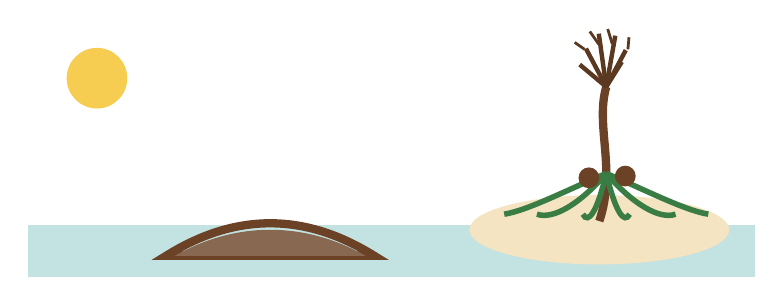
\begin{tikzpicture}[scale=1.1]
    \fill[sun!70] (-3.4,1.6) circle (0.35);
    \fill[ocean!25] (-4.2,-0.7) rectangle (4.2,-0.1);
    % 椰子島
    \fill[sand] (2.4,-0.15) ellipse (1.5 and 0.4);
    \begin{scope}[shift={(2.4,-0.05)}]\upsidedowntree\end{scope}
    % 獨木舟
    \draw[line width=3pt, coconut] (-2.6,-0.45) .. controls (-1.8,0.05) and (-1.0,0.05) .. (-0.2,-0.45) -- cycle;
    \fill[coconut!80] (-2.5,-0.45) .. controls (-1.8,-0.05) and (-1.0,-0.05) .. (-0.3,-0.45) -- cycle;
  \end{tikzpicture}
  \end{center}
\end{frame}

\begin{frame}{椰子國}
  \centering
  \vspace{0.1em}
  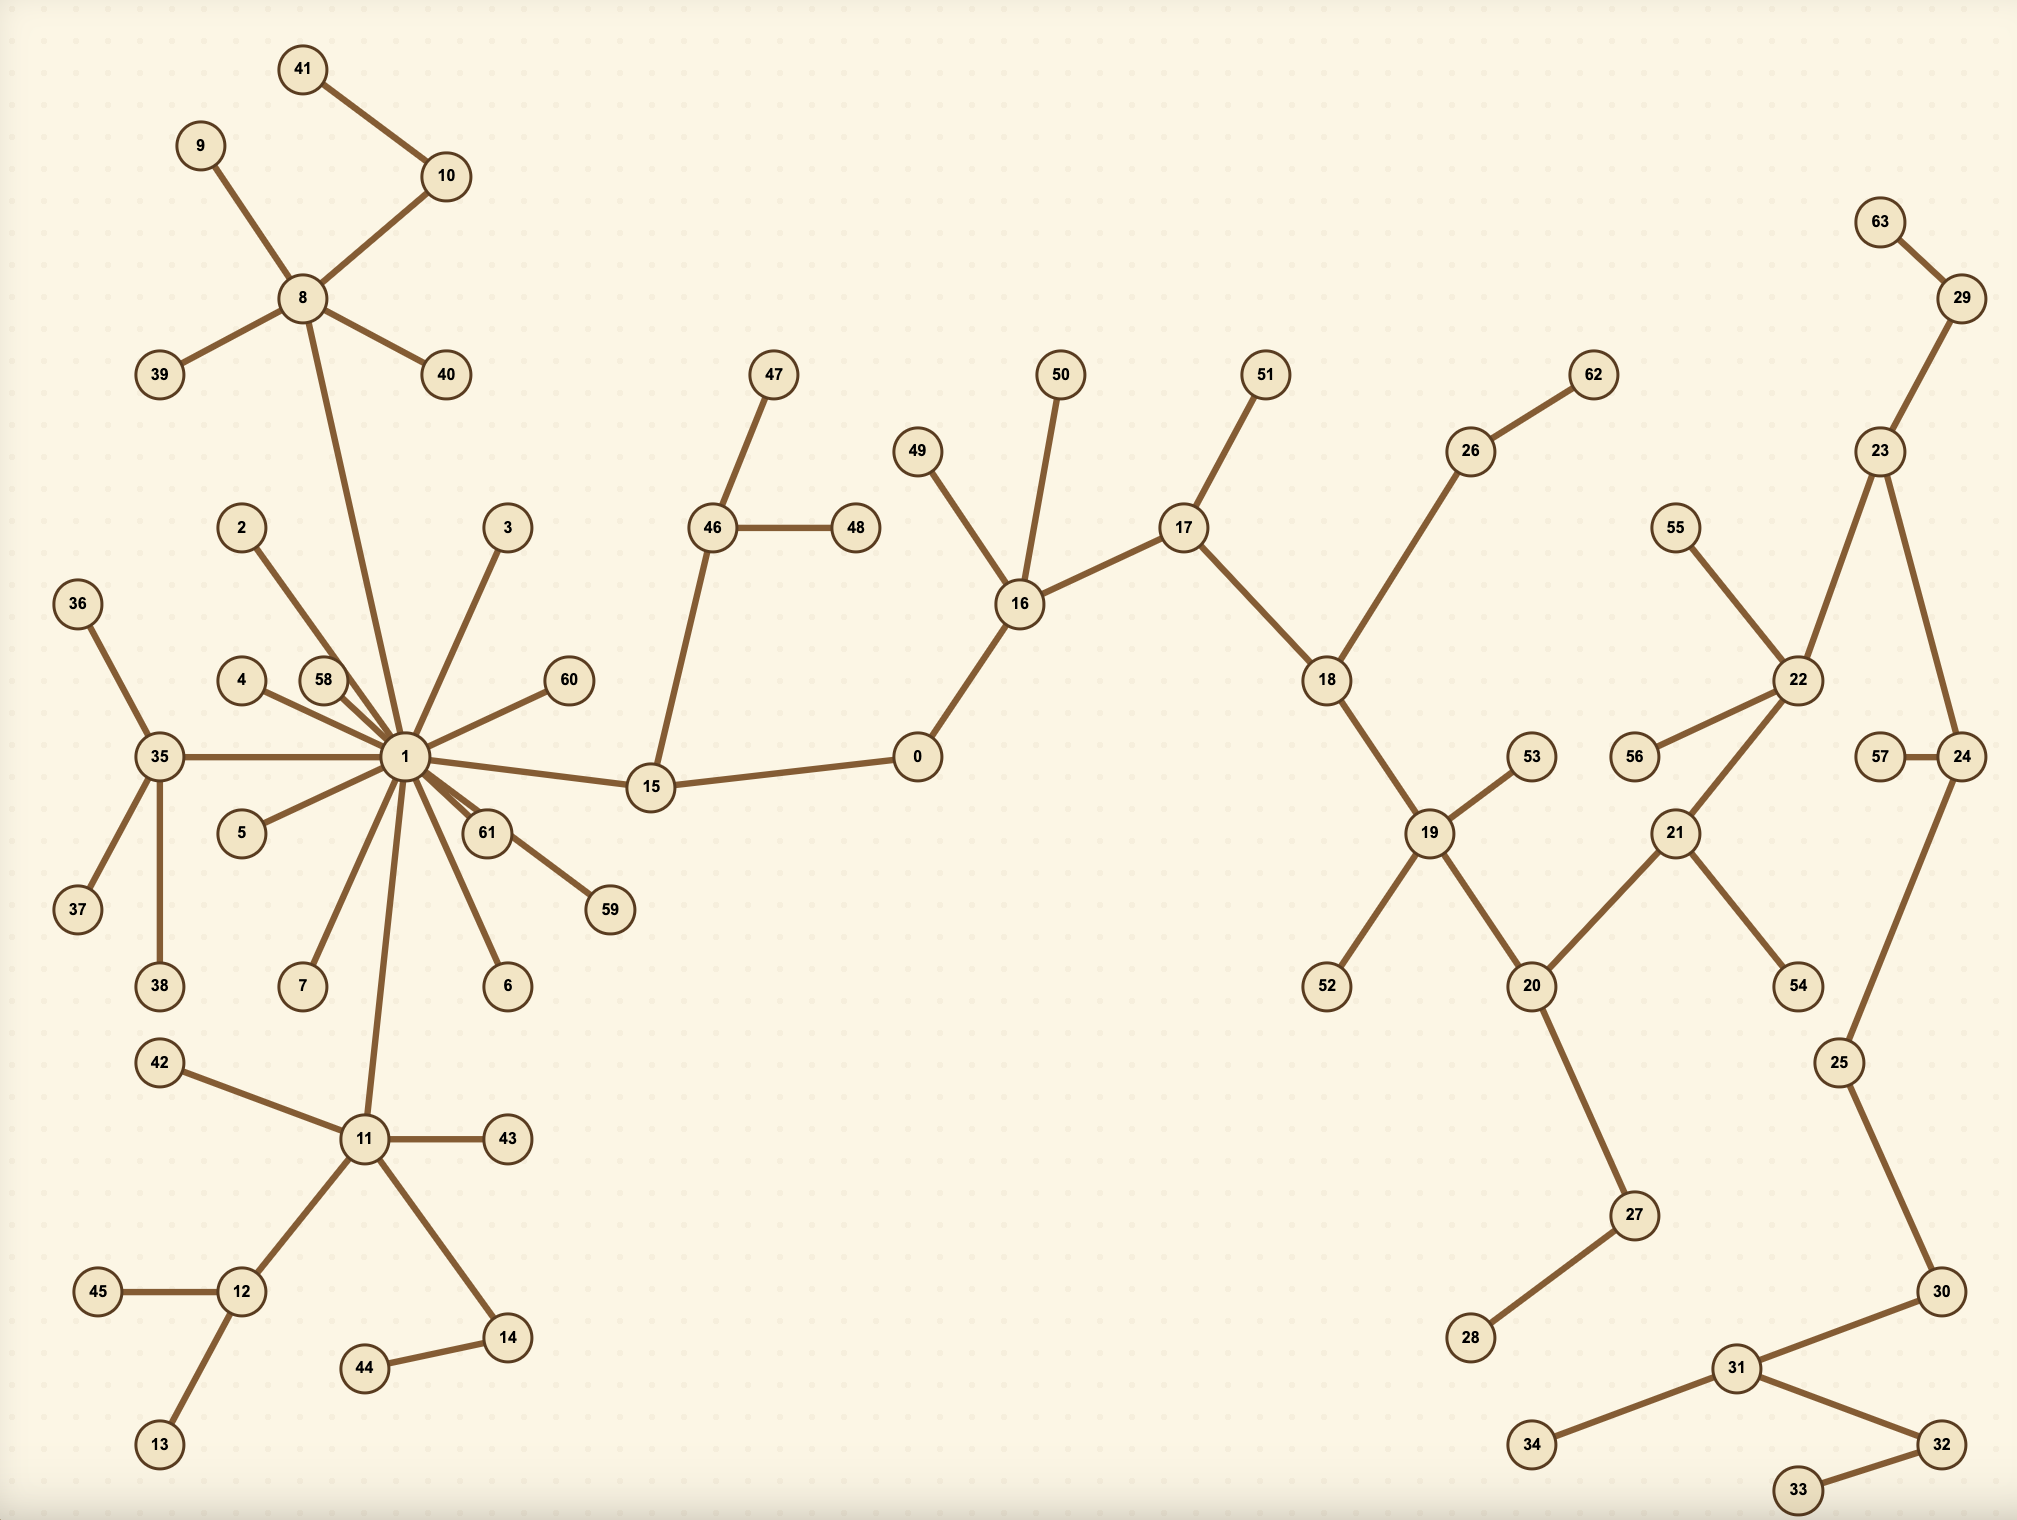
\includegraphics[width=0.55\textwidth]{coconut.png}\\[0.2em]
  {\footnotesize\textcolor{coconut!70!black}{
  這時椰子國的地圖。每個圈圈代表一顆椰子樹！椰子樹間有\textbf{步道}，椰子島民只能在步道間行走。}}
  \vspace{0.3em}
\end{frame}

\begin{frame}{藏寶遊戲}
  \begin{itemize}
    \item 胖椰在其中一棵樹下埋下了\textbf{寶藏}。
    \item 瘦椰跟胖椰在玩遊戲，他的目標是找到寶藏。
      \item 每一回合，瘦椰會選擇一棵椰子樹挖寶藏。
        \item 如果挖到寶藏，遊戲結束！
        \item 如果沒有挖到寶藏，胖椰要給瘦椰\textbf{提示}：胖椰會選擇一棵椰子樹，並跟瘦椰說：比起你剛剛選的椰子樹，這棵離寶藏比較近。
  \end{itemize}
\end{frame}

\begin{frame}{藏寶遊戲}
  \begin{itemize}
    \item 「近」的定義：
    \item 定義兩個椰子樹 $A$ 跟 $B$ 間的「距離」為：透過椰子島上的步島從 $A$ 走到 $B$，需要經過的最少步道數量。
    \item 胖椰要選的椰子樹，它離寶藏的「距離」要嚴格比瘦椰挖寶藏的地方離寶藏的「距離」來得小。
  \end{itemize}
\end{frame}

\begin{frame}{藏寶遊戲 - 範例}
  \centering
  \vspace{0.1em}
  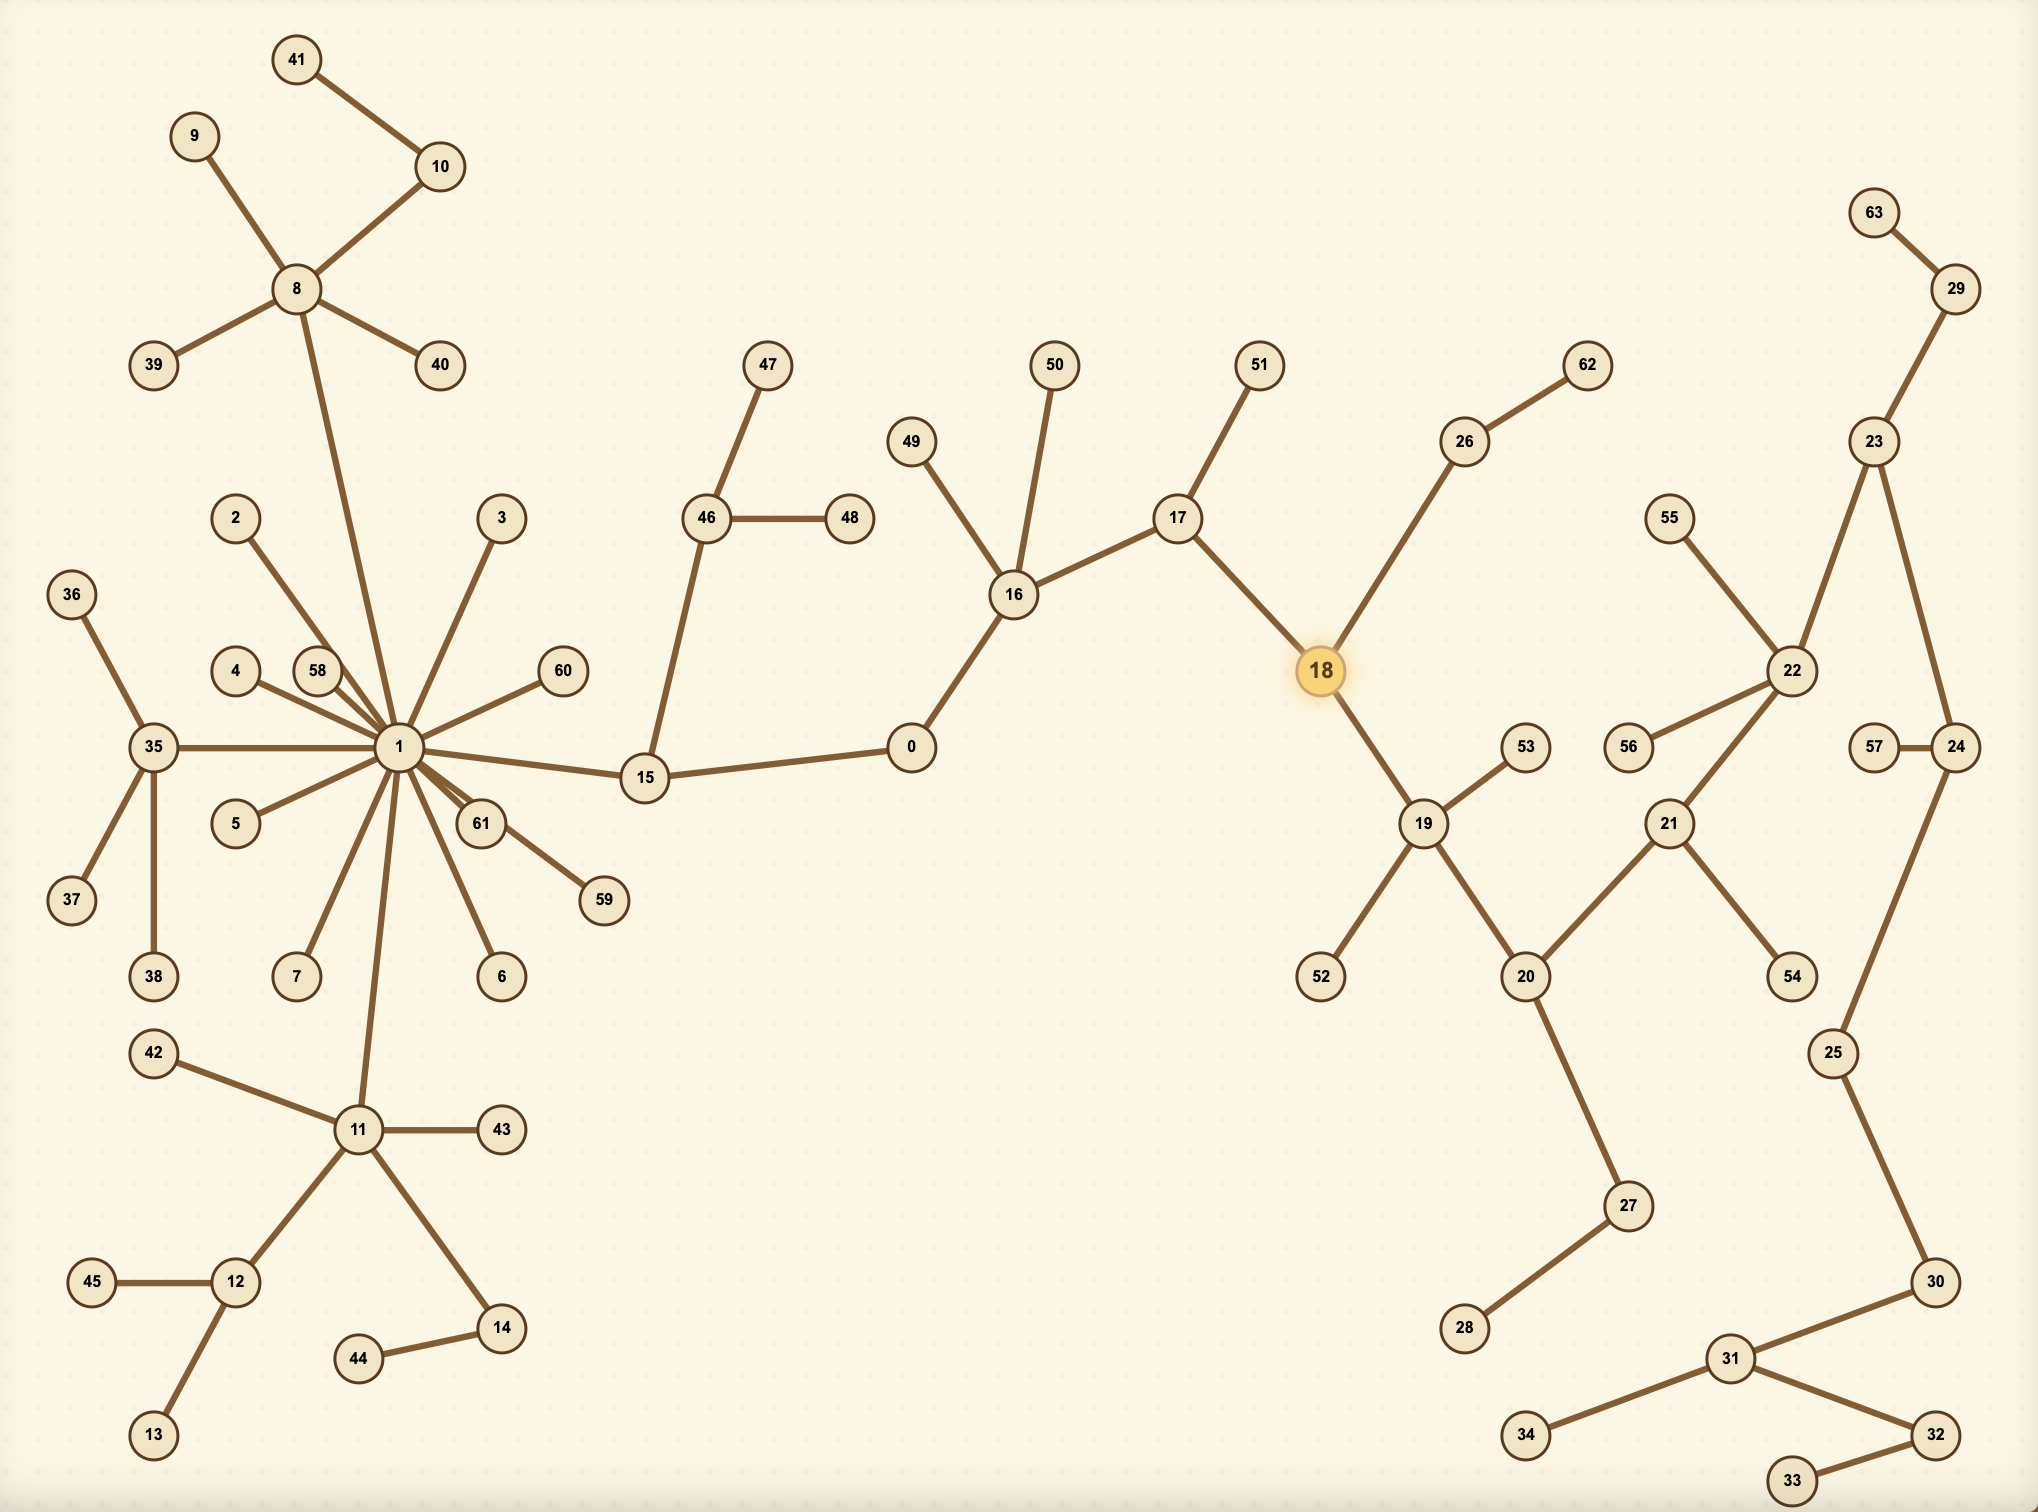
\includegraphics[width=0.55\textwidth]{coconut_treasure_2.png}\\[0.2em]
  {\footnotesize\textcolor{coconut!70!black}{
  胖椰選擇在 18 號樹下藏寶藏。}}
  \vspace{0.3em}
\end{frame}

\begin{frame}{藏寶遊戲 - 範例}
  \centering
  \vspace{0.1em}
  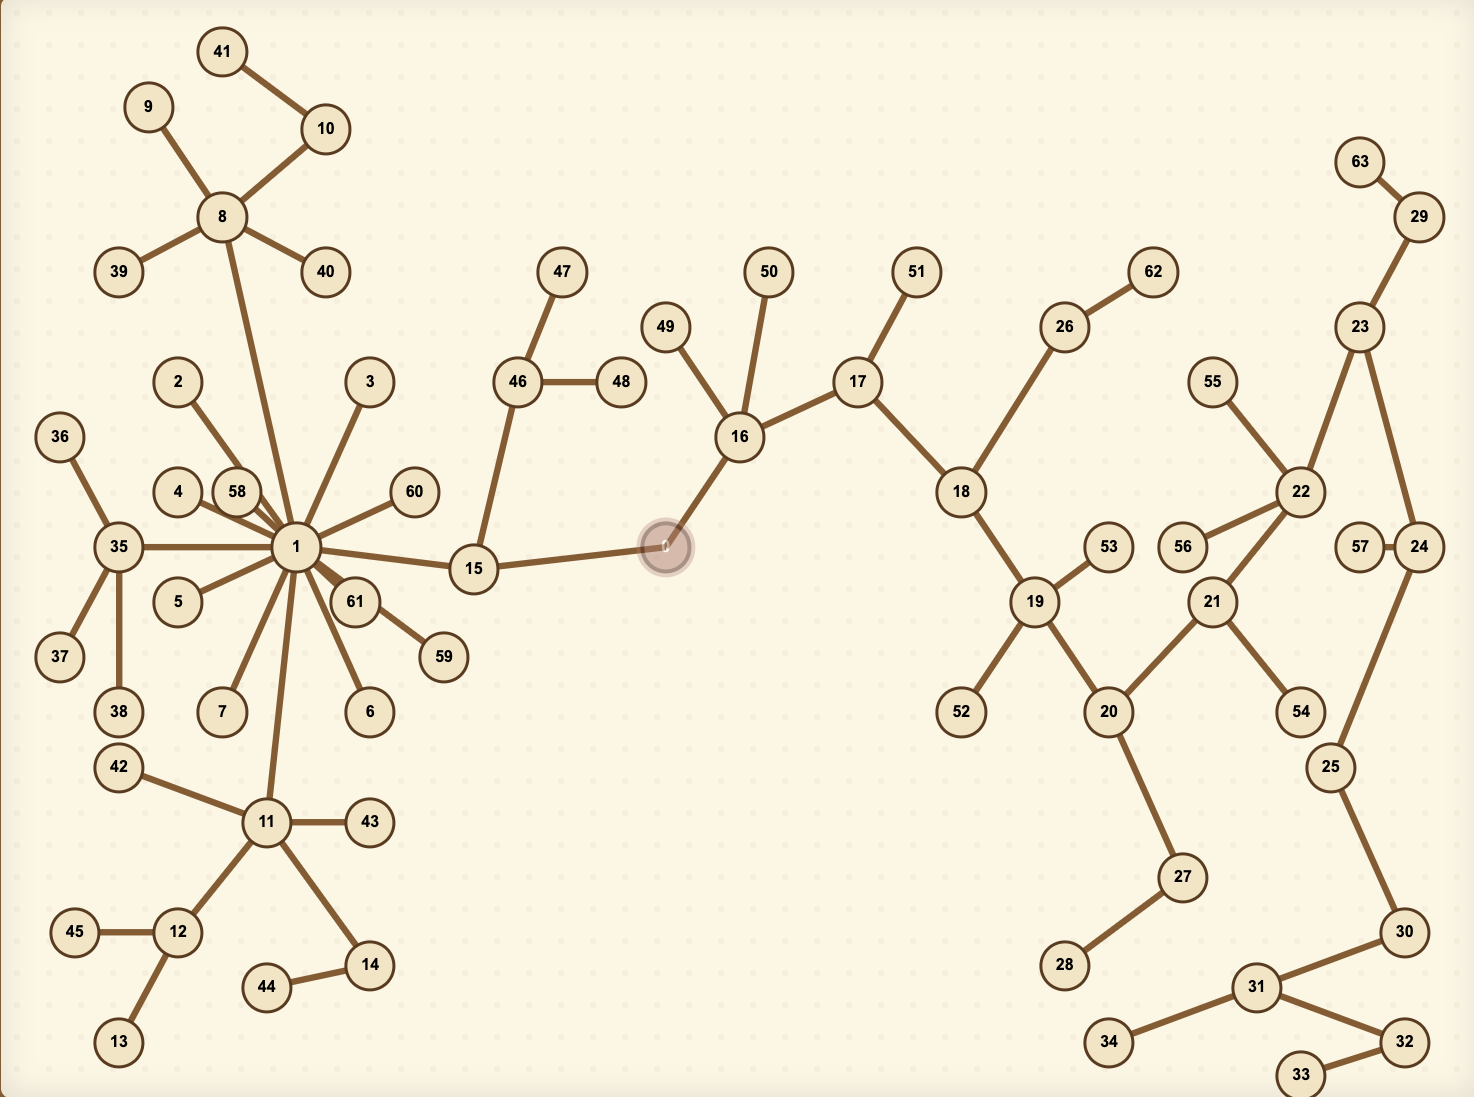
\includegraphics[width=0.6\textwidth]{coconut_guess_2.png}\\[0.2em]
  {\footnotesize\textcolor{coconut!70!black}{
  瘦椰猜測寶藏在 0 號樹下。}}
  \vspace{0.3em}
\end{frame}

\begin{frame}{藏寶遊戲 - 範例}
  \centering
  \vspace{0.1em}
  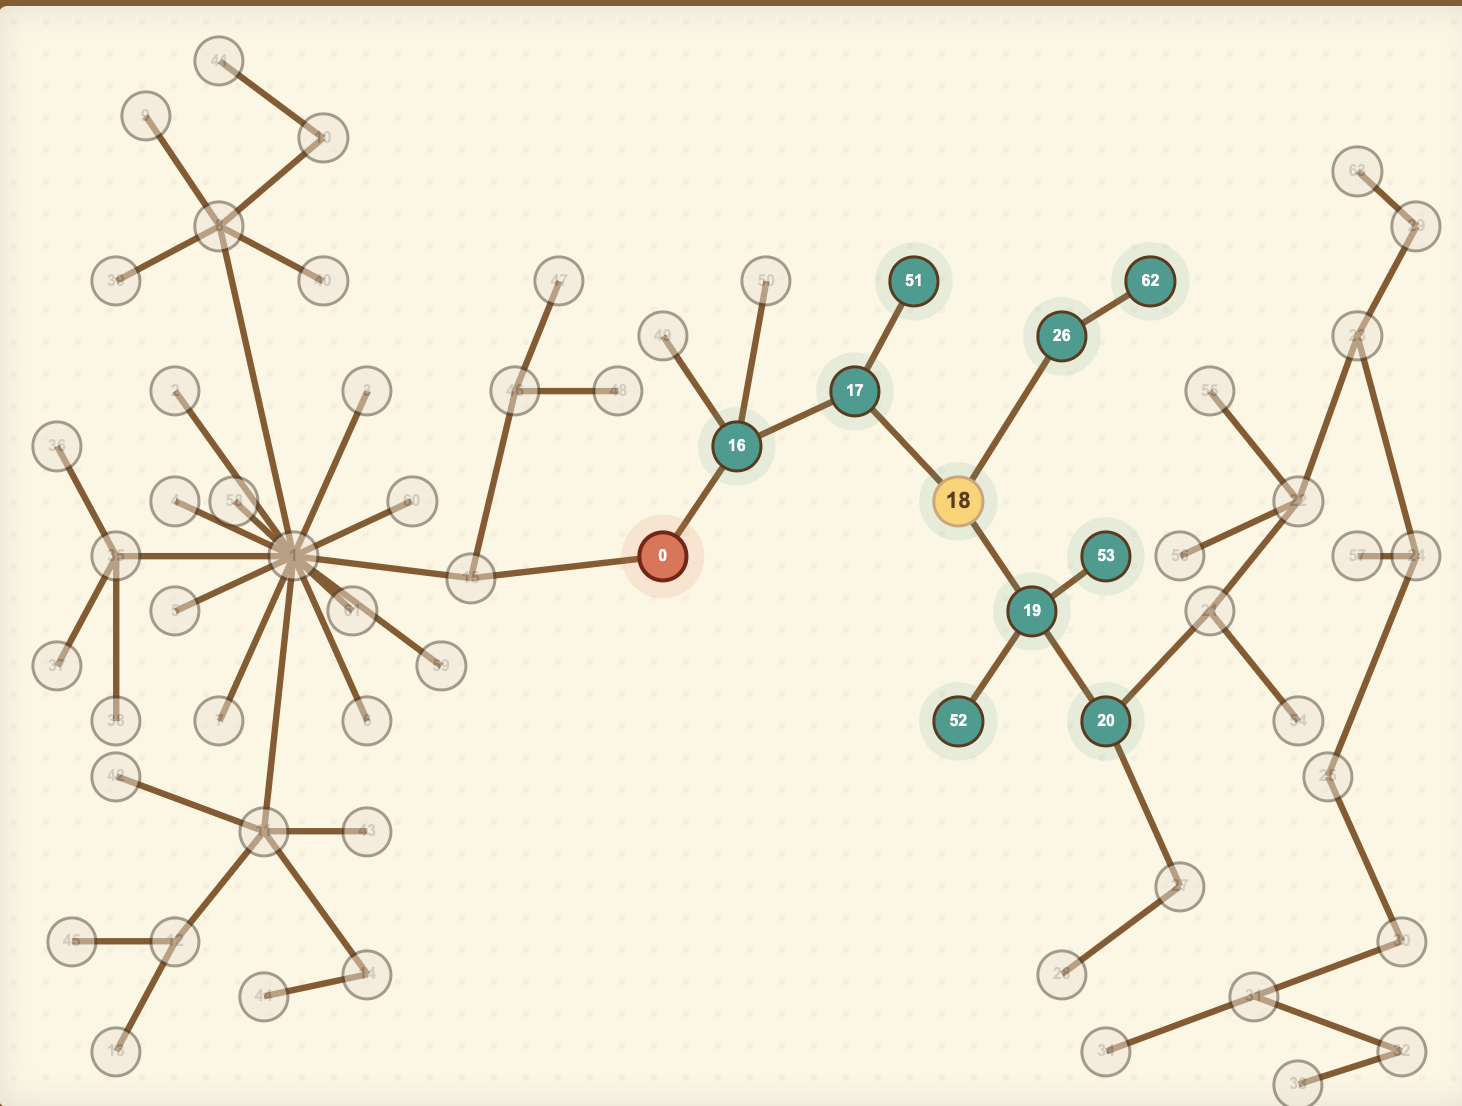
\includegraphics[width=0.57\textwidth]{coconut_reply_2.png}\\[0.2em]
  {\footnotesize\textcolor{coconut!70!black}{
  比起 0 號樹，綠色、黃色標示的樹離寶藏（18 號樹）更近。胖椰要選一棵樹給瘦椰提示，他選擇 17 號樹。}}
  \vspace{0.3em}
\end{frame}

\begin{frame}{藏寶遊戲 - 目標}
  \begin{itemize}
    \item 因為挖寶藏很累，瘦椰想要在最少回合內挖到寶藏。
    \item 因為看瘦椰挖土很好笑，胖椰想要讓回合數越多越好。
  \end{itemize}
\end{frame}

\begin{frame}{藏寶遊戲 - 目標}
  \begin{itemize}
    \item 兩隊中，一隊會先擔任瘦椰（\textbf{進攻隊}），另一對擔任胖椰（\textbf{防守隊}）。
    \item 進攻隊目標是猜越少回合越好，防守隊目標是守越多回合越好。
    \item 結束後，兩隊攻守交換。
    \item 挖最少椰子數的隊伍獲勝！
  \end{itemize}
\end{frame}

\begin{frame}{回合流程}
  \begin{itemize}
    \item 請兩隊各一個人用電腦進入關主傳在頻道中的關卡連結。
    \item 先給大家 3 分鐘討論戰術。
    \item 防守隊先選一棵椰子樹藏寶藏。
    \item 接著每回合：
      \item 進攻隊選一棵椰子樹猜測，時限 30 秒。
      \item 防守隊選一棵椰子樹回答，時限 30 秒。
      \item 如果 30 秒結束，還沒有做出決定的話，系統會幫你們隊隨機挑選一個合法的回答。
      % \item 希望組內能輪流操控電腦，大家都有玩遊戲的機會。
    \item 前面有一些椰子國的地圖，大家可以拿幾張地圖在上面規劃戰術。
  \end{itemize}
\end{frame}

\begin{frame}{藏寶遊戲 - 第二回合}
  \begin{itemize}
    \item 當你們玩的興高采烈時，椰子議會通過了預算案，在 15 號椰子樹和 28 號椰子樹中間興建了一座橋！
    \item 瘦椰和胖椰一樣想要在新的椰子國地圖上面玩藏寶遊戲，但加上了這座橋，一切都變複雜了...
  \end{itemize}
\end{frame}

\begin{frame}{藏寶遊戲 - 第二回合}
   \centering
  \vspace{0.1em}
  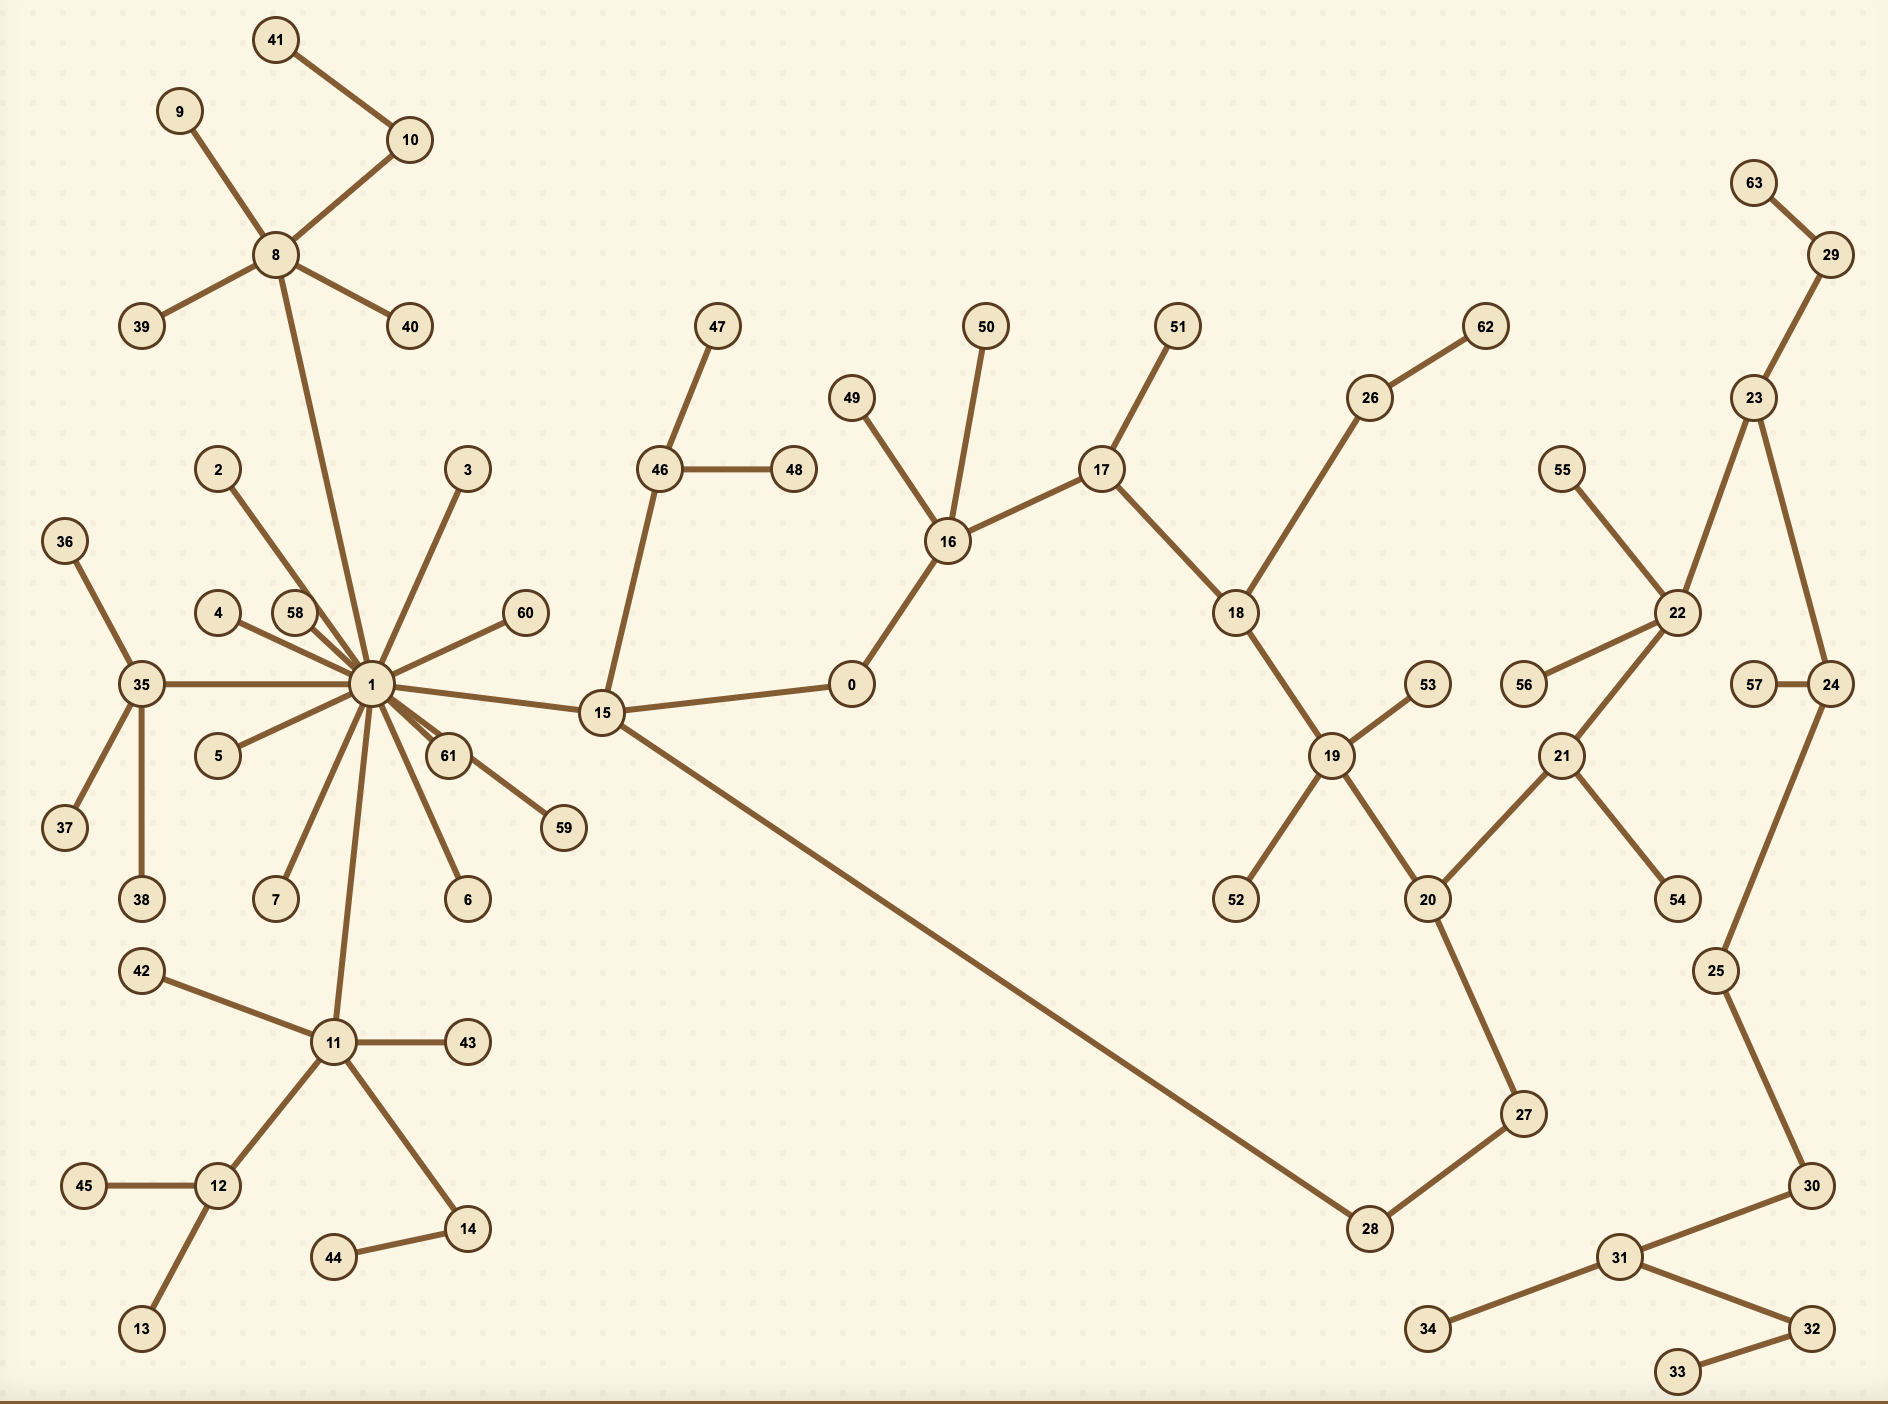
\includegraphics[width=0.57\textwidth]{coconut_jellyfish.png}\\[0.2em]
  {\footnotesize\textcolor{coconut!70!black}{
  新的椰子國地圖。}}
  \vspace{0.3em}
\end{frame}

\end{document}